Most usage data is collected as an activity stream with varying levels of supporting detail. In Figure~\ref{fig:theoretical} we present an abstraction of a typical activity stream. It includes a timestamp, followed by the activity, appended with (often anonymous) details concerning that activity. We can apply this model to the examples discussed earlier. For instance, the Mylyn Monitor's interaction event corresponds to a row in our theoretical model. It includes a timestamp (i.e., StartDate), an activity description (i.e., Kind, OriginId), and additional information (i.e., StructureHandle, StructureKind). Similarly, the CodingSpectator example includes a timestamp (i.e., stamp), an activity description (i.e., id), and a much larger set of additional information (i.e., code-snippet, selection, selection-in-code-snippet, etc.). Because these and other usage data activity streams can easily be described using our abstraction we will refer to it as we describe data analysis techniques.


%TODO: Rewrite/Adapt/Remove this paragraph now that it's been integrated

%What do they look like

%include theoretical example

%several concrete examples (codingsepctator, Sando, Eclipse study)

%Software systems often keep a record about what event was completed (or not) in the form of a log file. The information collected in the log file is often used for diagnostic purposes. If a system failure occurs, the logs for that period can be inspected to see which sequence of events were executed by the system and what were the values for the dynamic information in those events. Each log line can be traced back to a particular line of code where the method to log this information was called. Hene, we can get complete information on what events were executed. The log message store information about the branches taken by that particular instance of execution and the values for variables in the code. Due to these reasons, the information in the log file is collected as a serially ordered flat text file. In short, a log file is a collection of log lines, with each of them having information about a single event, its time of execution and the dynamic information about variable values. Note that each log line may span across multiple lines, but provides information to distinct two adjacent log lines.



\begin{figure*}[t]
 \centering
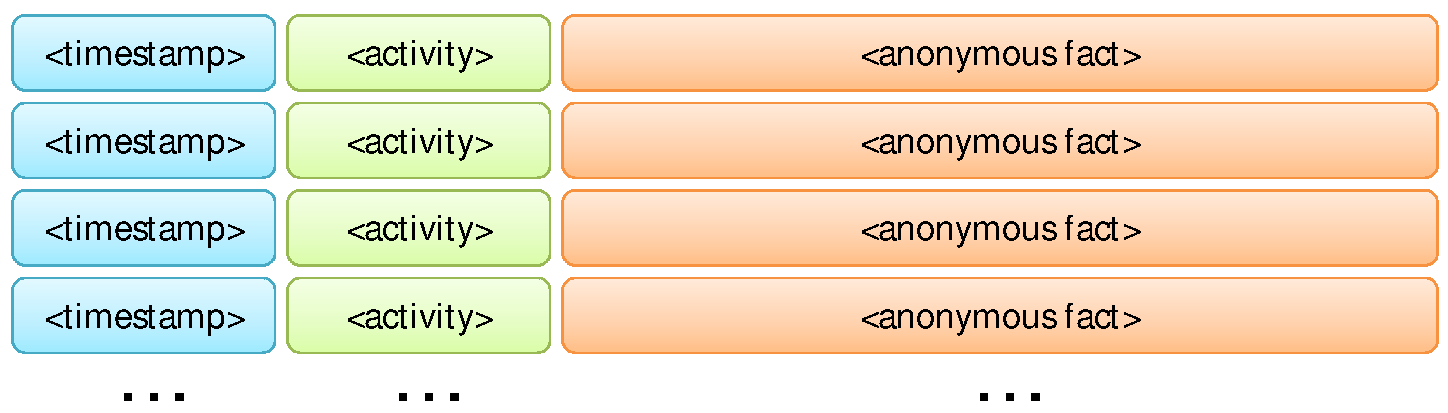
\includegraphics[width=1\columnwidth]{../Graphics/activityLogTheoretical.pdf}
\caption{Abstract model of developer activity streams.}
\label{fig:theoretical}
\end{figure*}



%\begin{figure*}[t]
 %\centering
%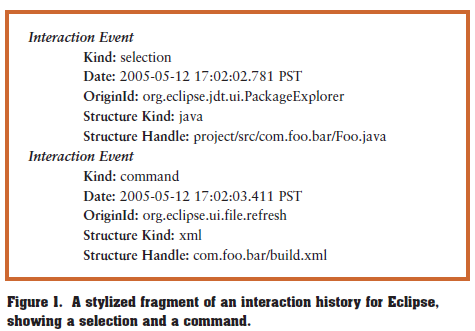
\includegraphics[width=0.5\columnwidth]{AnalyzingUsageData/activityEvent}
%\caption{Activities as Captured in an Eclipse Usage Data Study}
%\label{fig:activity}
%\end{figure*}
%
%\begin{figure*}[t]
 %\centering
%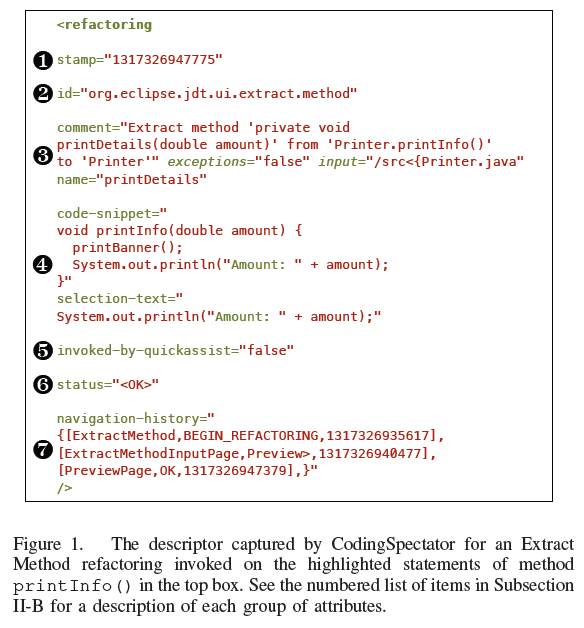
\includegraphics[width=0.5\columnwidth]{AnalyzingUsageData/codingSpectator}
%\caption{Activities as Captured in a CodingSpectator Study of Refactoring Events}
%\label{fig:activit}
%\end{figure*}

